\textbf{Implementering af sensorer}
For at implementere de forskellige sensorer, herunder EMG og accelerometre, skal ADC'en opsættes så den kan opsamle fra 3 kanaler. Dette gøres ved at opsætte dette i PSoC, som er illustreret på \autoref{fig:PSoC_sensor}.

\begin{figure}[H]
\centering
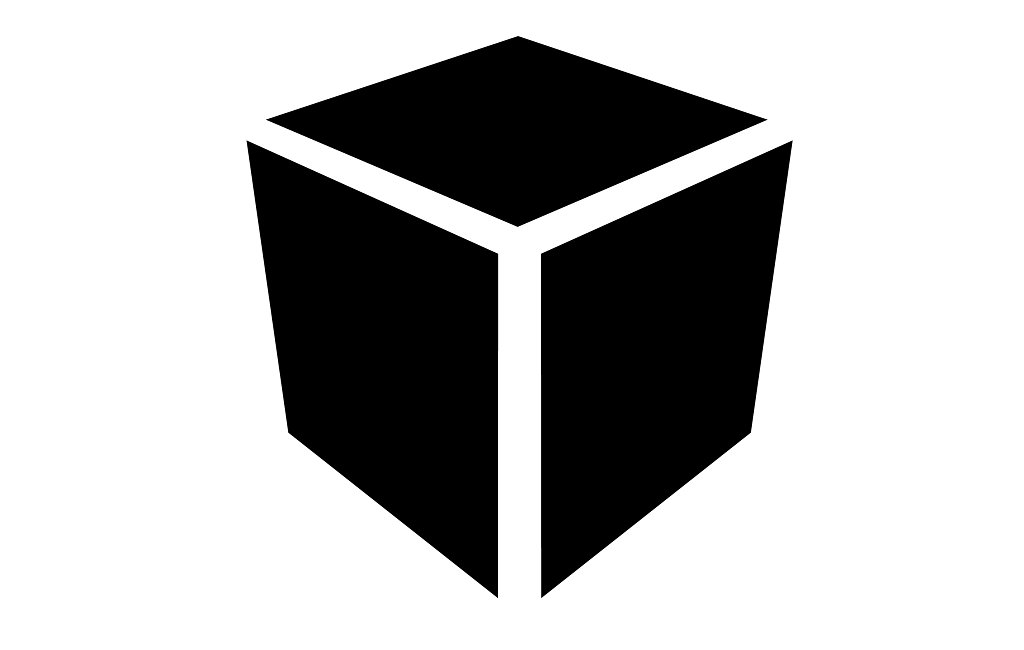
\includegraphics[width=0.85\textwidth]{figures/blackbox}
\caption{her skal der stå et eller andet smart....}
\label{fig:PSoC_sensor}
\end{figure}

For at test om signalet bliver opsamlet som forventet i PSoC visualiseres dette i MATLAB og sammenlignes med målingerne for pilotforsøget \autoref{sec:pilotforsoeget}. Resultaterne fra opsamling af de forskellige sensorer fremgår af \autoref{fig:PSoC_sensor1}.

\begin{figure}[H]
\centering
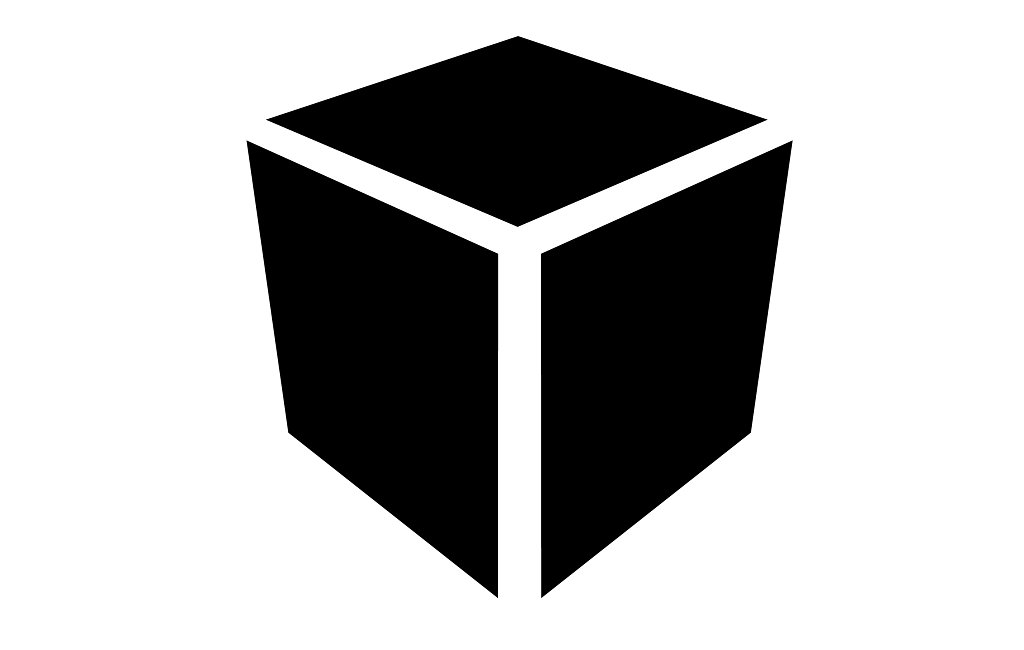
\includegraphics[width=0.85\textwidth]{figures/blackbox}
\caption{her skal der stå et eller andet smart....}
\label{fig:PSoC_sensor1}
\end{figure}